\chapter[CoNVaDING: Single Exon Variation Detection in NGS data]{CoNVaDING: Single Exon Variation Detection in Targeted NGS Data}
\chaptermark{CoNVaDING: CNV detection in NGS data}
\label{chap:CoNVaDING}

{ \Large \leftwatermark{
		\put(-67,-66.5){ 1 }
		\put(-67,-91.5){ 2 }
		\put(-76.5,-125){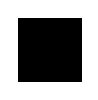
\includegraphics[scale=0.8]{img/thumbindex.eps}} \put(-67,-116.5){ {\color{white} 3 }}
		\put(-67,-141.5){ 4 }
		\put(-67,-166.5){ 5 }
		\put(-67,-191.5){ 6 }
		\put(-67,-216.5){ 7 }
		\put(-67,-241.5){ 8 }
		\put(-67,-266.5){ 9 }
		\put(-67,-291.5){ 10 }
		\put(-67,-316.5){ 11 }
	} \rightwatermark{
		\put(350.5,-66.5){ 1 }
		\put(350.5,-91.5){ 2 }
		\put(346.5,-125){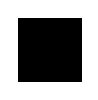
\includegraphics[scale=0.8]{img/thumbindex.eps}} \put(350.5,-116.5){ {\color{white} 3 }}
		\put(350.5,-141.5){ 4 }
		\put(350.5,-166.5){ 5 }
		\put(350.5,-191.5){ 6 }
		\put(350.5,-216.5){ 7 }
		\put(350.5,-241.5){ 8 }
		\put(350.5,-266.5){ 9 }
		\put(350.5,-291.5){ 10 }
		\put(350.5,-316.5){ 11 }
}}

\hfill \underline{Human Mutation} 2016;37(5):457-464.

\hfill DOI: \href{https://doi.org/10.1002/humu.22969}{10.1002/humu.22969}

\hfill PubMed ID: \href{https://www.ncbi.nlm.nih.gov/pubmed/26864275}{26864275}

\newpage

\noindent
L.F. Johansson\textsuperscript{1,2,*}, F. van Dijk\textsuperscript{1,2,*}, E.N. de Boer\textsuperscript{1}, K.K. van Dijk-Bos\textsuperscript{1}, J.D. Jongbloed\textsuperscript{1}, A.H. van der Hout\textsuperscript{1}, H. Westers\textsuperscript{1}, R.J. Sinke\textsuperscript{1}, M.A. Swertz\textsuperscript{1,2}, R.H. Sijmons\textsuperscript{1},B. Sikkema-Raddatz\textsuperscript{1}  \\

\noindent
1. University of Groningen, University Medical Center Groningen, Department of Genetics, Groningen, The Netherlands\\
2. University of Groningen, University Medical Center Groningen, Genomics Coordination Center, Groningen, The Netherlands\\


\noindent
Received 2015 Nov 26; Accepted revised manuscript 2016 Jan 27; Published online 2016 Feb 10.
\\~\\
* Contributed equally


\section*{Abstract}\label{abstract}
We have developed a tool for detecting single exon copy-number variations (CNVs) in targeted next-generation sequencing data: CoNVaDING (Copy Number Variation Detection In Next-generation sequencing Gene panels).
CoNVaDING includes a stringent quality control (QC) metric, that excludes or flags low-quality exons. 
Since this QC shows exactly which exons can be reliably analyzed and which exons are in need of an alternative analysis method, CoNVaDING is not only useful for CNV detection in a research setting, but also in clinical diagnostics. 
During the validation phase, CoNVaDING detected all known CNVs in high-quality targets in 320 samples analyzed, giving 100\% sensitivity and 99.998\% specificity for 308,574 exons. 
CoNVaDING outperforms existing tools by exhibiting a higher sensitivity and specificity and by precisely identifying low-quality samples and regions. 

\section{Introduction}\label{introduction}
Several methods for detecting exon deletion and duplication using next-generation sequencing (NGS) have been reported for whole genome \cite{Zhao_2013,Gilissen_2014,Francioli_2014} and whole gene sequencing data \cite{Wang_2014}. 
With the exception of those using read depth approaches, these methods rely on information from sequence reads spanning the breakpoints. 
For targeted NGS data, however, only a read depth approach can be successfully applied \cite{Tan_2014}. 
Existing tools using this approach are XHMM \cite{Fromer_2012}, CoNIFER \cite{Krumm_2012}, CONTRA \cite{Li_2012}, and CODEX \cite{Jiang_2015}. 
All four consider all control samples equally informative even though there are sample to sample variations caused by differences in PCR and capturing efficiency, which lead to variations in coverage patterns that complicate the determination of expected read depths \cite{Aird_2011}\cite{Zhao_2013}. 
In the four existing tools, this increases the risk of false- negative (FN) or false-positive (FP) results for exons with a high read depth variation, giving either a low sensitivity and specificity for single exon copy-number variation (CNV) detection or limiting the analysis to detection of variations that span multiple exons. 
This has meant that, until now, additional experiments were needed to identify single exon CNVs, including multiplex ligation-dependent probe amplification (MLPA) \cite{Schouten_2002}, Q-PCR \cite{Ebenazer_2013}, or array comparative hybridization \cite{Vasson_2013}. 
These additional experiments are, however, costly and usually only applied to genes known to frequently harbor deletions or duplications. 
To overcome this limitation, we have developed CoNVaDING, an analysis tool that not only detects single (and multiple) exon CNVs with high sensitivity and specificity, but also provides quality metrics for each sample that distinguish high-quality samples and targets from low-quality ones with a high risk of producing FP or FN results.

\section{Material and Methods}

\subsection{General Workflow CoNVaDING}
The CoNVaDING analysis consists of several steps to determine whether a deletion or duplication is present. 
CoNVaDING focuses on specified target regions (Fig. \ref{fig:CoNVaDING_Fig1}A) and utilizes control samples captured with the same gene panel for a read depth comparison. 
A strategy unique for CoNVaDING is that out of a set of available control samples, it selects only samples with a coverage pattern that is most similar to that of the sample analyzed (Fig. \ref{fig:CoNVaDING_Fig1}C). \
The selected control samples are therefore most informative for this specific sample. 
CoNVaDING then normalizes the data in two different ways in parallel in order to enable comparison between the sample and the control samples. The first normalization uses all targets or all autosomal targets within the sample (Fig. \ref{fig:CoNVaDING_Fig1}B) and the second uses all targets of the same gene (Fig. \ref{fig:CoNVaDING_Fig1}D). 
Based on the normalized data, the ratio of the normalized average read depth of the sample to that of the controlsanda distribution analysis using a Z-score are calculated for each target (Fig. \ref{fig:CoNVaDING_Fig1}E). 
Based on the calculated ratio and distributions, a prediction is made for each target to determine whether a CNV is present or not (Fig. \ref{fig:CoNVaDING_Fig1}F). 
The mathematical formulas used are described in the Supplemental methods.


\begin{figure}
	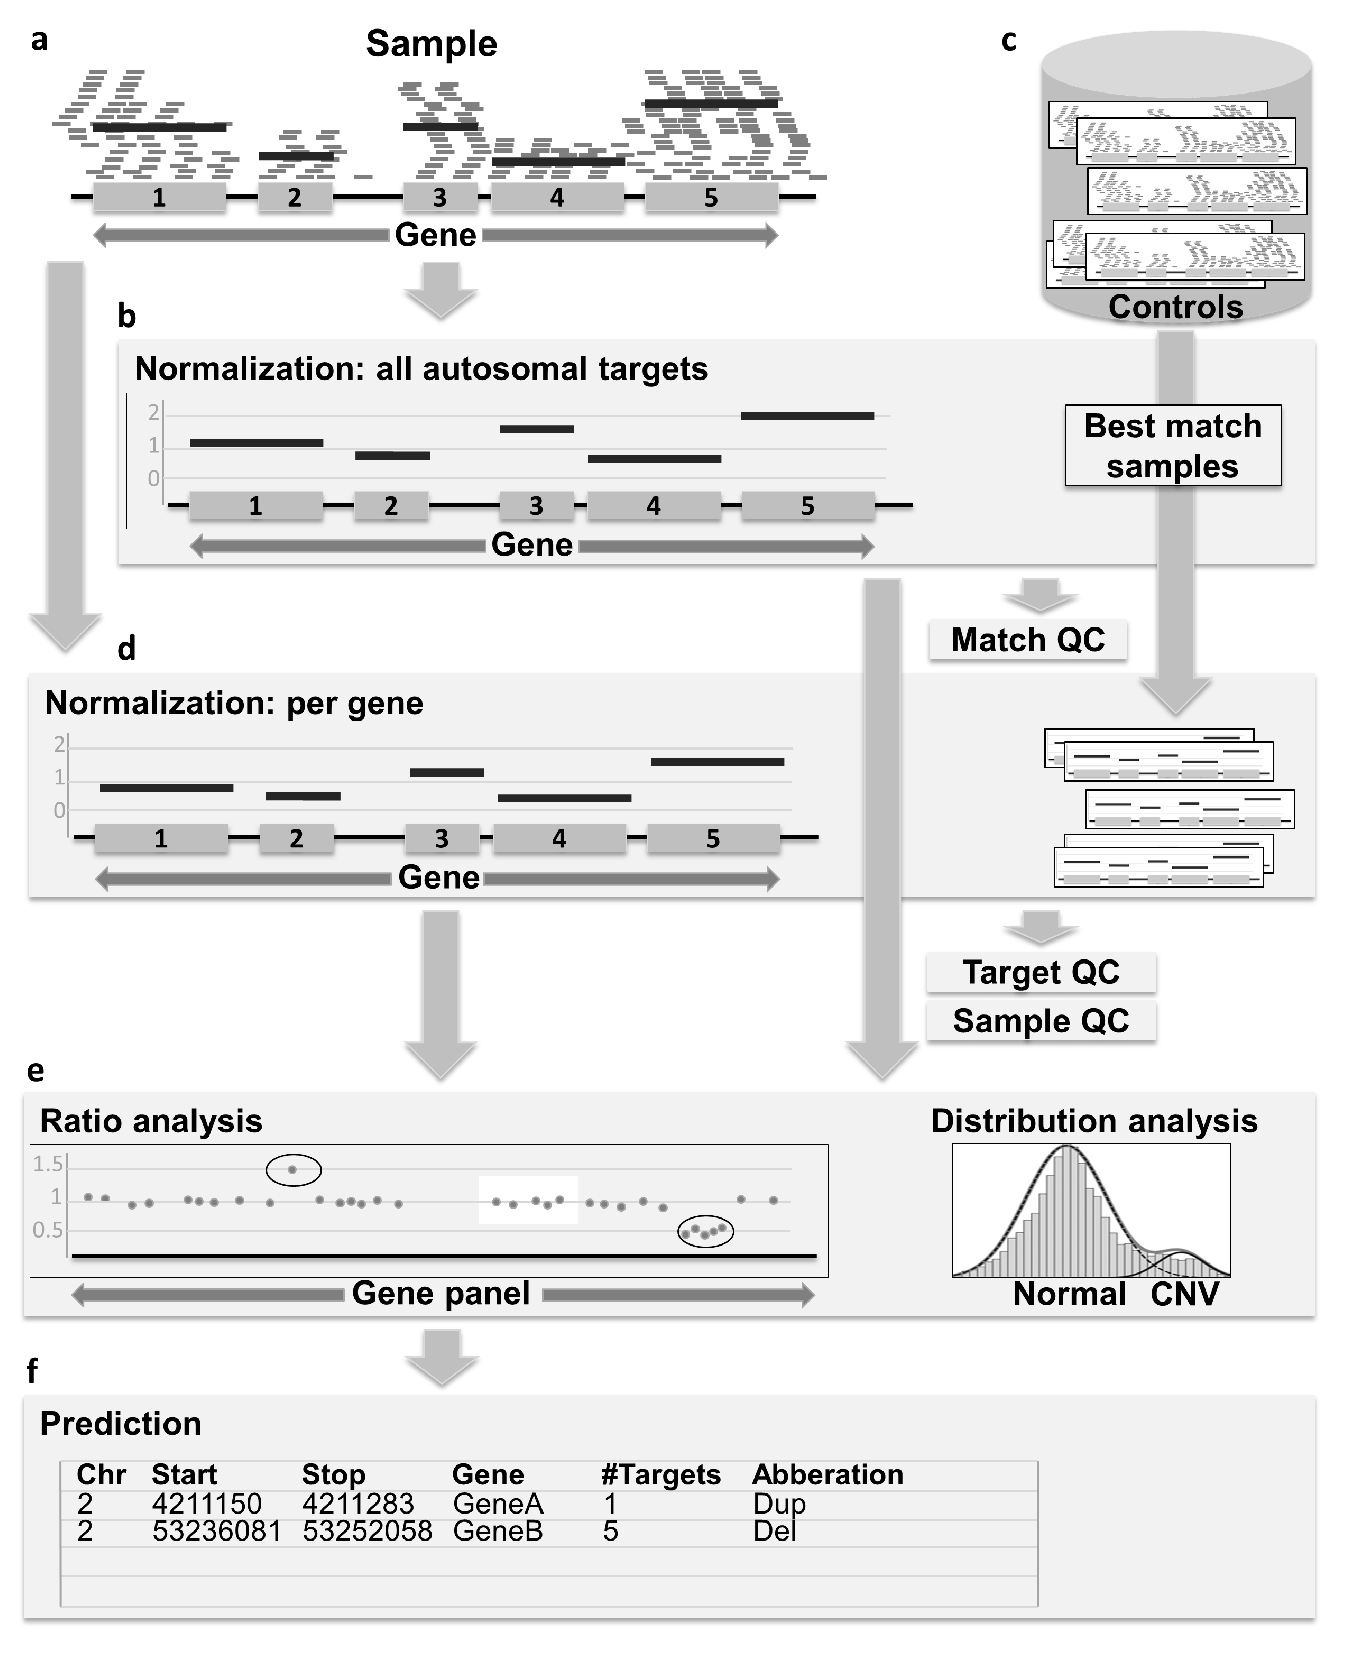
\includegraphics[width=1.0\linewidth]{img/CoNVaDING_Fig1}
	\caption[CoNVaDING workflow]{Caption next page.}
	\label{fig:CoNVaDING_Fig1}
\end{figure}
\addtocounter{figure}{-1}
\begin{figure}
\caption[]{(Previous page.) CoNVaDING workflow. A: For each specified target region, the average coverage is calculated for the analyzed sample. B: The sample is normalized using the average coverages of all autosomal targets. C: Out of a set of possible control samples, the samples showing the most similar coverage pattern are selected as control samples. The Match QC shows how well the control samples match the analyzed sample. D: All targets are alternatively normalized using the average coverages of targets belonging to the same gene. E: Based on the normalizations, a ratio and a distribution analysis are performed, showing the relative difference of the average coverages of the targets of the sample compared with those of the control samples. Target QC and Sample QC metrics are calculated showing the variability of each target and the complete sample. F: Based on the ratio and distribution analysis, a copy-number variation (CNV) prediction is made.}
\end{figure}

\subsection{Input Data}
CoNVaDING analysis starts with a list of targets that specify chromosome, start and stop position of the target and the exact gene the target belongs to. 
For each sample and the possible control samples, a BAM file containing aligned reads is also needed \cite{Li_2009}. 
Typically, targets specify the exonic regions ofwhich the gene panel consists of, or a subset thereof. 
After an optional removal of sequence duplicates, for each BAMfile, of all targets in the sample and in the possible control samples, the average depth of coverage is calculated (Fig. \ref{fig:CoNVaDING_Fig1}A).

\subsection{Control Group Selection}
CoNVaDING makes use of a set of possible control samples that should be produced using the same type of sample preparation and sequencing as the test sample. 
The control samples with the most similar overall coverage patterns are selected using a “match score” for each possible control sample. 
This match score is calculated by first correcting all samples for total read number difference, that is, dividing the average depth of coverage of the target by the mean average depth of coverage of all (autosomal) targets (typeAnormalization) (Fig. \ref{fig:CoNVaDING_Fig1}B). 
Subsequently, the absolute difference between the sample and each possible control sample is calculated for each target. 
For each possible control sample, the absolute differences are sorted from smallest to largest and the average absolute difference of the center 95\% targets, the match score, is calculated. 
A lower match score indicates a more similar overall coverage pattern and thus a more suitable control sample. The control samples with the lowest match scores are selected for further analysis (Fig. \ref{fig:CoNVaDING_Fig1}C). 
A minimum of 30 control samples is needed for analysis. 
An example of the characteristics of the selected control groups for two samples is shown in Figure \ref{fig:CoNVaDING_Fig2}.


\begin{figure}[!ht]
	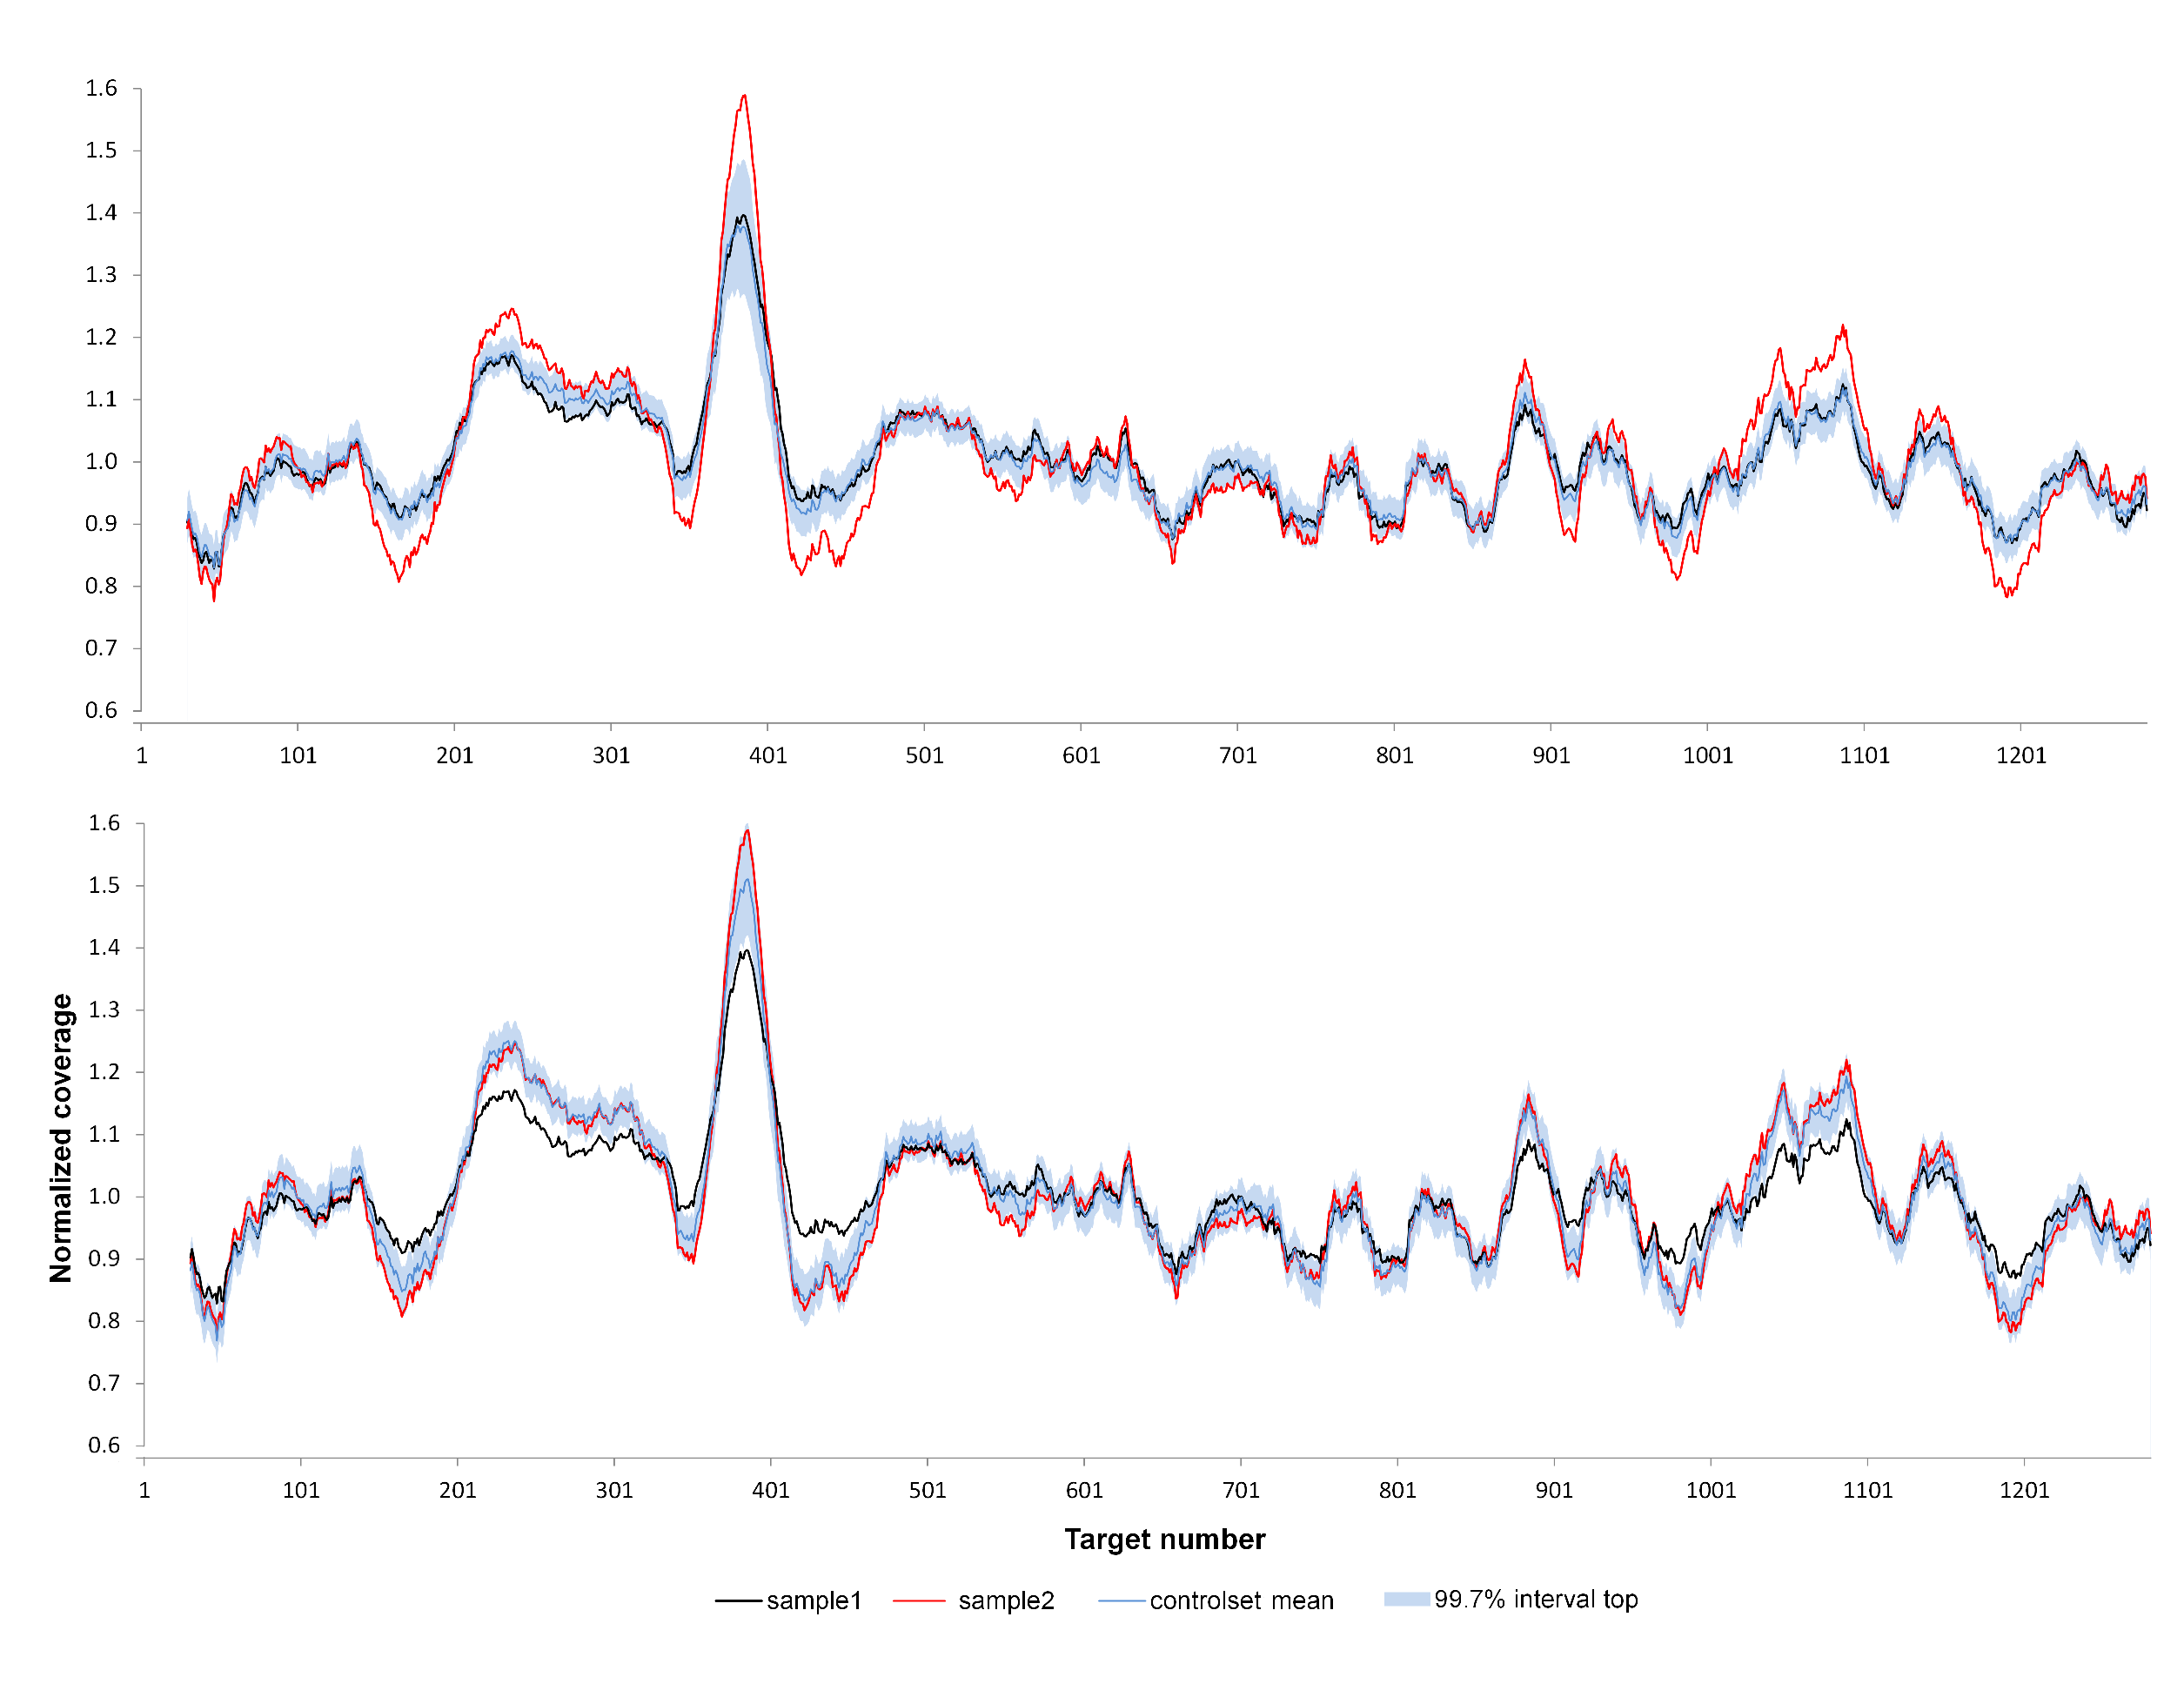
\includegraphics[width=1.0\linewidth]{img/CoNVaDING_Fig2}
	\caption[CoNVaDING match control group]{Both graphs show the moving average of the normalized coverage over 30 targets of two test samples (sample 1 [black continuous line] and sample 2 [red line line]) and the mean control group value of the 30 best matching normalized control samples (blue line line) with the 99.7\% confidence interval (light blue area area). In graph (A), the best-fitting control samples for sample 1 are selected as control group and in graph (B) the best-fitting control samples for sample 2 are selected. Both test samples fitwithin the 99.7\% confidence interval of their own best matching control group, but compared with the 99.7\% confidence interval of the other control group, there are overrepresented and underrepresented regions.}
	\label{fig:CoNVaDING_Fig2}
\end{figure}

\subsection{CNV Prediction Score Calculation}
After the control group selection, the selected control samples are used as a reference set. 
All samples are normalized to enable comparison between samples. Two types of analysis, the ratio score analysis and the distribution score analysis, are performed to determine determine the relative difference between the sample of interest and the selected control samples. 
Results of both calculations are combined and, together with quality metrics, are used to predict the presence of a CNV. 
Normalization within the sample is done in two different ways.
The first (type A normalization) is the normalization using all (autosomal) targets (Fig. \ref{fig:CoNVaDING_Fig1}B). 
The second (type B normalization) alternatively normalizes the read number of the targets by dividing the average depth of coverage of the target of interest by the mean average depth of coverage of all targets belonging to the same gene as the target (Fig. \ref{fig:CoNVaDING_Fig1}D).

\subsubsection{Ratio score}
The ratio score shows the ratio of the read depth of the sample to the expected read depth (Fig. \ref{fig:CoNVaDING_Fig1}E). 
This score is calculated for each target by dividing the type A normalized depth of coverage by the average type A normalized depth of coverage in the selected control samples. 
If no deletion or duplication is present, the sample of interest is expected to have the same normalized average depth of coverage as the selected control samples, a condition indicated by ratio scores close to 1.0. 
Deletions and duplications are expected to have a ratio of \textapprox0.5 and \textapprox1.5, respectively. Default cut-offs are set at a ratio below 0.65 for deletions and a ratio above 1.4 for duplications. 
Ratios below 0.10 or above 1.75 indicate homozygous deletions or amplifications, respectively. This is in concordancewith the cut-offs used in MLPA \cite{MRC_Holland_2014}, with the exception of the duplication threshold, which we increased from 1.3 to a more stringent 1.4 to improve specificity. Targets with an average coverage of 0 are excluded from further analysis.


\subsubsection{Distribution score}
The distribution score calculates the number of standard deviations by which the read depth of a target in the sample analyzed differs from the mean read depth of the control samples (Fig. \ref{fig:CoNVaDING_Fig1}E). 
For both type-A- and type-B-normalized targets, a Z-score is calculated by subtracting the average normalized depth of coverage of the selected control samples fromthe normalized depth of coverage for the sample and dividing the result by the standard deviation of the normalized depth of coverage of the selected control samples. 
If the Z-score is higher than three (i.e., three standard deviations or more from the average), the distribution score is indicative of a duplication. 
If the Z-score is lower than minus three, the distribution score is indicative of a deletion. 
When 30 or more control samples are selected, the normalized average coverage of a target in the selected control samples is expected to have a normal distribution. The optimal number of best matching control samples to select is dependent on the number of possible control samples and the consistency of the coverage patterns.

\subsection{Quality Control Metrics}
CoNVaDING provides three different quality control (QC) metrics: Match QC shows how well the coverage pattern of the sample fits the selected control samples, Sample QC shows the variability between all targets within the sample, and Target QC shows the variability for each target within the control samples.

\subsubsection{Match QC}
To determine whether the selected control samples have a similar coverage pattern to that of the sample of interest, a Match QC score is calculated. This score is equal to the mean of the match scores of the selected control samples. 
Match QC is provided for troubleshooting purposes and can be used to determine how repre- sentative the selected control samples are for the sample analyzed. 
No thresholds are specified, but a higherMatch QC score indicates a less representative control group.

\subsubsection{Sample QC}
For the sample of interest, a QC metric is calculated that makes the variability in the sample explicit. 
First, the informative targets are selected by excluding the standard low-quality targets, because they would erroneously lower sample quality. 
Targets for which there is no coverage in all possible control samples and type A-normalized targets in which more control samples than allowed (default: over 20\%) show a Z-score outside the confidence intervals (default 99.7\%) are considered low quality. 
For each target of the sample of interest, a second normalization is done by dividing the type A-normalized depth of coverage of the target in the sample by the average type A-normalized depth of coverage of that target in all selected control samples. 
The double normalized informative targets are sorted from low-to-high normalized depth of coverage. 
Finally, the Sample QC metric is calculated by using the average and standard deviation of the center 95\% of these targets to calculate a coefficient of variation.

\subsubsection{Target QC}
For each target, a QC metric is calculated. This metric specifies the variability of the specific target in the control samples and consists of the coefficient of variation of the type A-normalized depth of coverage for the selected control samples. 
Targets with a higher coefficient of variation thanallowed (default setting 0.10) are labeled as low quality.

\subsection{CNV Calling}
In short, the output of CoNVaDING consists of three lists: a high-sensitivity “longlist” containing all CNV calls regardless of quality, a high-specificity “shortlist,” using Target QC values of the sample analyzed for filtering, and a high-specificity “final list” using Target QC information of all control samples to filter CNVs. 
CNV calling is performed based on the combined information from ratio and distribution scores (Fig. \ref{fig:CoNVaDING_Fig1}F).
For a target to be labeled as a CNV, the type A ratio and distribution scores and the type B distribution score have tobe indicative of a deletion or a duplication. 
If two or more adjacent targets are labeled as a CNV, only one of the three scores has to be indicative for a deletion or a duplication. 
Rows of consecutive deleted or duplicated targets are considered as a single CNV. Because large deletions can disrupt the type B distribution score, a secondary calling strategy is applied to detect CNVs that comprise a half or more of a gene. 
If half or more of the targets of a specific gene are indicative of a deletion or a duplication for both the type A ratio and distribution score, those targets are labeled as a CNV. 
A CNV is labeled as a homozygous deletion or amplification only when this is indicated by all targets of the CNV. 
All the CNVs are added to the CNV longlist.

\subsubsection{Filtered targets}
Not all targets are suitable for reliable CNV detection. 
The high variability of low-quality targets decreases sensitivity and specificity. 
Therefore, CNV calls consisting only of low-quality targets are filtered fromthe longlist to create the shortlist. 
To further increase specificity, targets that are often of a low quality within the control group are filtered out from the shortlist to create the final list. 
For this, all possible control samples are analyzed with their own respective best matching control samples. When the TargetQC fails for too many samples (default \textgreater20\%), the target is filtered. 
Samples or targets failing QC are not suitable for single exon CNV detection. 
However, CNVs spanning multiple exons that contain low-quality targets are still reliably detected as long as some of the targets pass Target QC.

\subsection{Implementation of CoNVaDING}
CoNVaDING is implemented in a Perl command line script that can be easily integrated into automated analysis pipelines (see Supplemental User Manual).
The software depends only on standardPerl packages and SAMtools \cite{Li_2009} for mean coverage calculations and duplicate marking. 
CoNVaDING software is available under the GNU GPL open source license and can be freely downloaded from \\
https://github.com/molgenis/CoNVaDING

\subsection{Validation of CoNVaDING}

\subsubsection{Patients/samples}
Samples were included retrospectively from the population of patients with cardiomyopathy and pulmonary arterial hypertension\footnote{In the original article wrongly the term 'artificial' was used instead of 'arterial'} (CM) (N = 200) or familiar cancer (FC) (N = 120) referred to the genetics department of the University Medical Center Groningen. 
Targeted NGS had been performed previously for SNP analysis using a panel consisting of 73 genes associated with FC (Supplemental Table S1) and a panel containing of 61 genes associated with CM (Supplemental Table S2). 
Positive control samples (N = 10) with a known CNV were randomly included for retrospective analysis. These CNVs were previously identified using MLPA in BRCA1 (2x del 1 exon, 1x dup 2 exons, 1x del 3 exons, 1x del 5 exons), EPCAM (1x del 2 exons), MSH2 (1xdel 1exon, 1x del 10 exons MSH2, and 2 exons EPCAM), MLH1 (1x del 1 exon), or PMS2 (1x del 3 exons). 
Except for the positive control samples, no prior CNV detection using MLPA was performed for these samples. 
Laboratory procedures were performed as described in Sikkema-Raddatz et al. (2013) \cite{Sikkema_Raddatz_2013} using a biotinylated cRNA probe solution, manufactured byAgilent Technologies (Agilent Technologies, Santa Clara, CA). 
All samples were sequenced 151 bp paired-end on an IlluminaMiseq sequencer (Illumina, San Diego, CA).

\subsubsection{Data analysis}
For each sample, the sequence data were aligned to the human reference genome build b37, as released by the 1000 Genomes Project \cite{Durbin_2010}, using BWA \cite{Li_2010}. 
Subsequently, duplicate readsweremarkedby Picard \cite{Picard_nd}. 
Using the Genome Analysis Toolkit (GATK) \cite{McKenna_2010}, realignment around insertions and deletions detected in the sequence data and in the 1000 Genomes Project pilot \cite{Durbin_2010} was performed, followed by base quality score recalibration. 
During the full process, the quality of the data was assessed by performing Picard, GATK Coverage, and custom scripts. This production pipeline was implemented using the MOLGENIS compute \cite{Byelas_2013} platform for job generation, execution, and monitoring. 
The resulting BAM files were used as input for CNV analysis. 
For CoNVaDING CNV detection, the 30 best matching samples were used as control samples. 
To assess the effect of coverage on the performance of CoNVaDING, the BAM file of each sample was randomly downsampled to an average coverage of autosomal targets of 100x and of 50x using SAMtools \cite{Li_2009}. 
For both the 100x and the 50x average coverage samples, a CoNVaDING analysis was performed as described above.

\subsection{Comparison to CoNIFER, XHMM, and CODEX}
To assess theperformance of our tool,we compared CoNVaDING with two well-evaluated CNV analysis tools for targeted NGS data that do not require a paired normal control sample \cite{Guo_2013,Magi_2013,Backenroth_2014,Tan_2014}: CoNIFER \cite{Krumm_2012} and XHMM \cite{Fromer_2012}. 
In addition, CODEX \cite{Jiang_2015}, a more recent CNV analysis tool, was included in the comparison. 
We optimized the settings of these tools to obtain the highest possible sensitivity and specificity using the following changes to their default settings. 
For CoNIFER in the analyze step, targets were combined on a virtual chromosome to ensure that enough targets were present to make analysis possible. Optimal singular value decomposition (svd) values were determined at 4 for the FC panel and at 10 for the CM panel. 
Samples with a standard deviation of the SVD-ZRPKM values (produced with the {-}{-}write\_sd parameter during the analyze step \cite{Krumm_2012b} exceeding 0.5 were treated as samples failing Sample QC.
This is in line with CoNIFER QC as describedin Krumm et al. (2012)\cite{Krumm_2012}. 
CNV calls in samples that passed Sample QC were interpreted as positive results. 
XHMM analysis yielded the best results using a CNV rate of 1x10\textsuperscript{–6} and a mean number of targets in CNV of 2. 
Filter settings during the matrix step \cite{Fromer_2012b} were set to 1000 for maxMeanSampleRD and 1500 for maxMeanTargetRD. 
For all other parameters default settings were used. 
Samples excluded during analysiswith the {-}{-}matrix {-}{-}excludeSamples parameter \cite{Fromer_2012b} were interpreted as samples failing Sample QC, whereas targets excluded during analysis with the {-}{-}matrix {-}{-}excludeTargets parameter \cite{Fromer_2012b} were interpreted as failing Target QC. 
We tested CODEX using default settings. 
CODEX sample QC checks for samples with a low on-target read count and target QC filters exons in case of a low coverage (median \textless20x), exon length (\textless20 bp), low mappability (\textless0.9),or an extreme GC content (outside the 20–80\% range). 
We ran CoNVaDING, CoNIFER, XHMM, and CODEX on all samples. For true positive (TP)/FP analysis, CNV calls detected by CoNIFER or XHMM and calls on the CoNVaDING final list in samples that passed Sample QC were also analyzed via MLPA. 
Due to a high number of CODEX calls, we did not perform MLPA on new calls and did not accurately determine specificity for CODEX. 
We also tested CONTRA \cite{Li_2012}, but did not detect any CNVs in our control samples, so we excluded CONTRA from further comparison. 
We have determined sensitivity and specificity for CoNVaDING, CoNIFER, XHMM, and CODEX by calculating TP, FP, FN, and true-negative (TN) results. 
Calls analyzed with MLPA were considered TP when confirmed and FP when MLPA did not show a CNV and the sample and targets passed QC. 
If a CNV was detected using MLPA and no CNV was detected in the NGS data and the sample and targets passed QC, the call was considered FN. 
All targets in which none of the tools detected a CNV were considered as TN results, because only rare CNVs are expected in the genes analyzed and thus there is a low apriori risk of there being a CNV.

\section{Results}\label{results}

\subsection{Validation of CoNVaDING}
The FC and CM panels consisted of 1,002 and 1,281 autosomal targets, respectively, for a total of 376,440 targets analyzed. The average coverage was 220x for FC samples and 487x for CM samples. 
Of the total number of samples, 93\% of FC and 92\% of CM samples passed CoNVaDING Sample QC. 
Of these, on average 916 (91\%) and 1,118 (87\%) targets passed Target QC for the FC and CM panel, respectively, resulting in 308,574 high-quality targets. 

CoNVaDING identified 15 CNVs in samples that passed Sample QC, 10 of which were confirmed with MLPA and labeled TP (Fig. \ref{fig:CoNVaDING_Fig3}A). 
Five had a normal MLPA result and were labeled FP (Fig. \ref{fig:CoNVaDING_Fig3}B). 
The TP CNVs included the seven BRCA1, EPCAM, and PMS2 positive control aberrations, as well as one extra finding in the FC panel, a 16 exon ALK duplication, and two extra findings in the CM panel, a deletion of the DSP gene (24 exons), and a 2 exon deletion in CTNNA3 (Supplemental Table S3). 
In the 10 positive control samples, the two MSH2 deletions were detected in a sample failing Sample QC. 
The MLH1 deletion was filtered out from the final list after failing Target QC. 
Thus, CoNVaDING had 100\% sensitivity and 99.998\% specificity for targets passing QC. 
The analysis speed of CoNVaDING was tested on the 200 CM samples, using a BED file specifying the targets, on a desktop PC. 
From average count file to final list all samples can be analyzed in less than 90 minutes using maximum 1 GB RAM.

\begin{figure}
	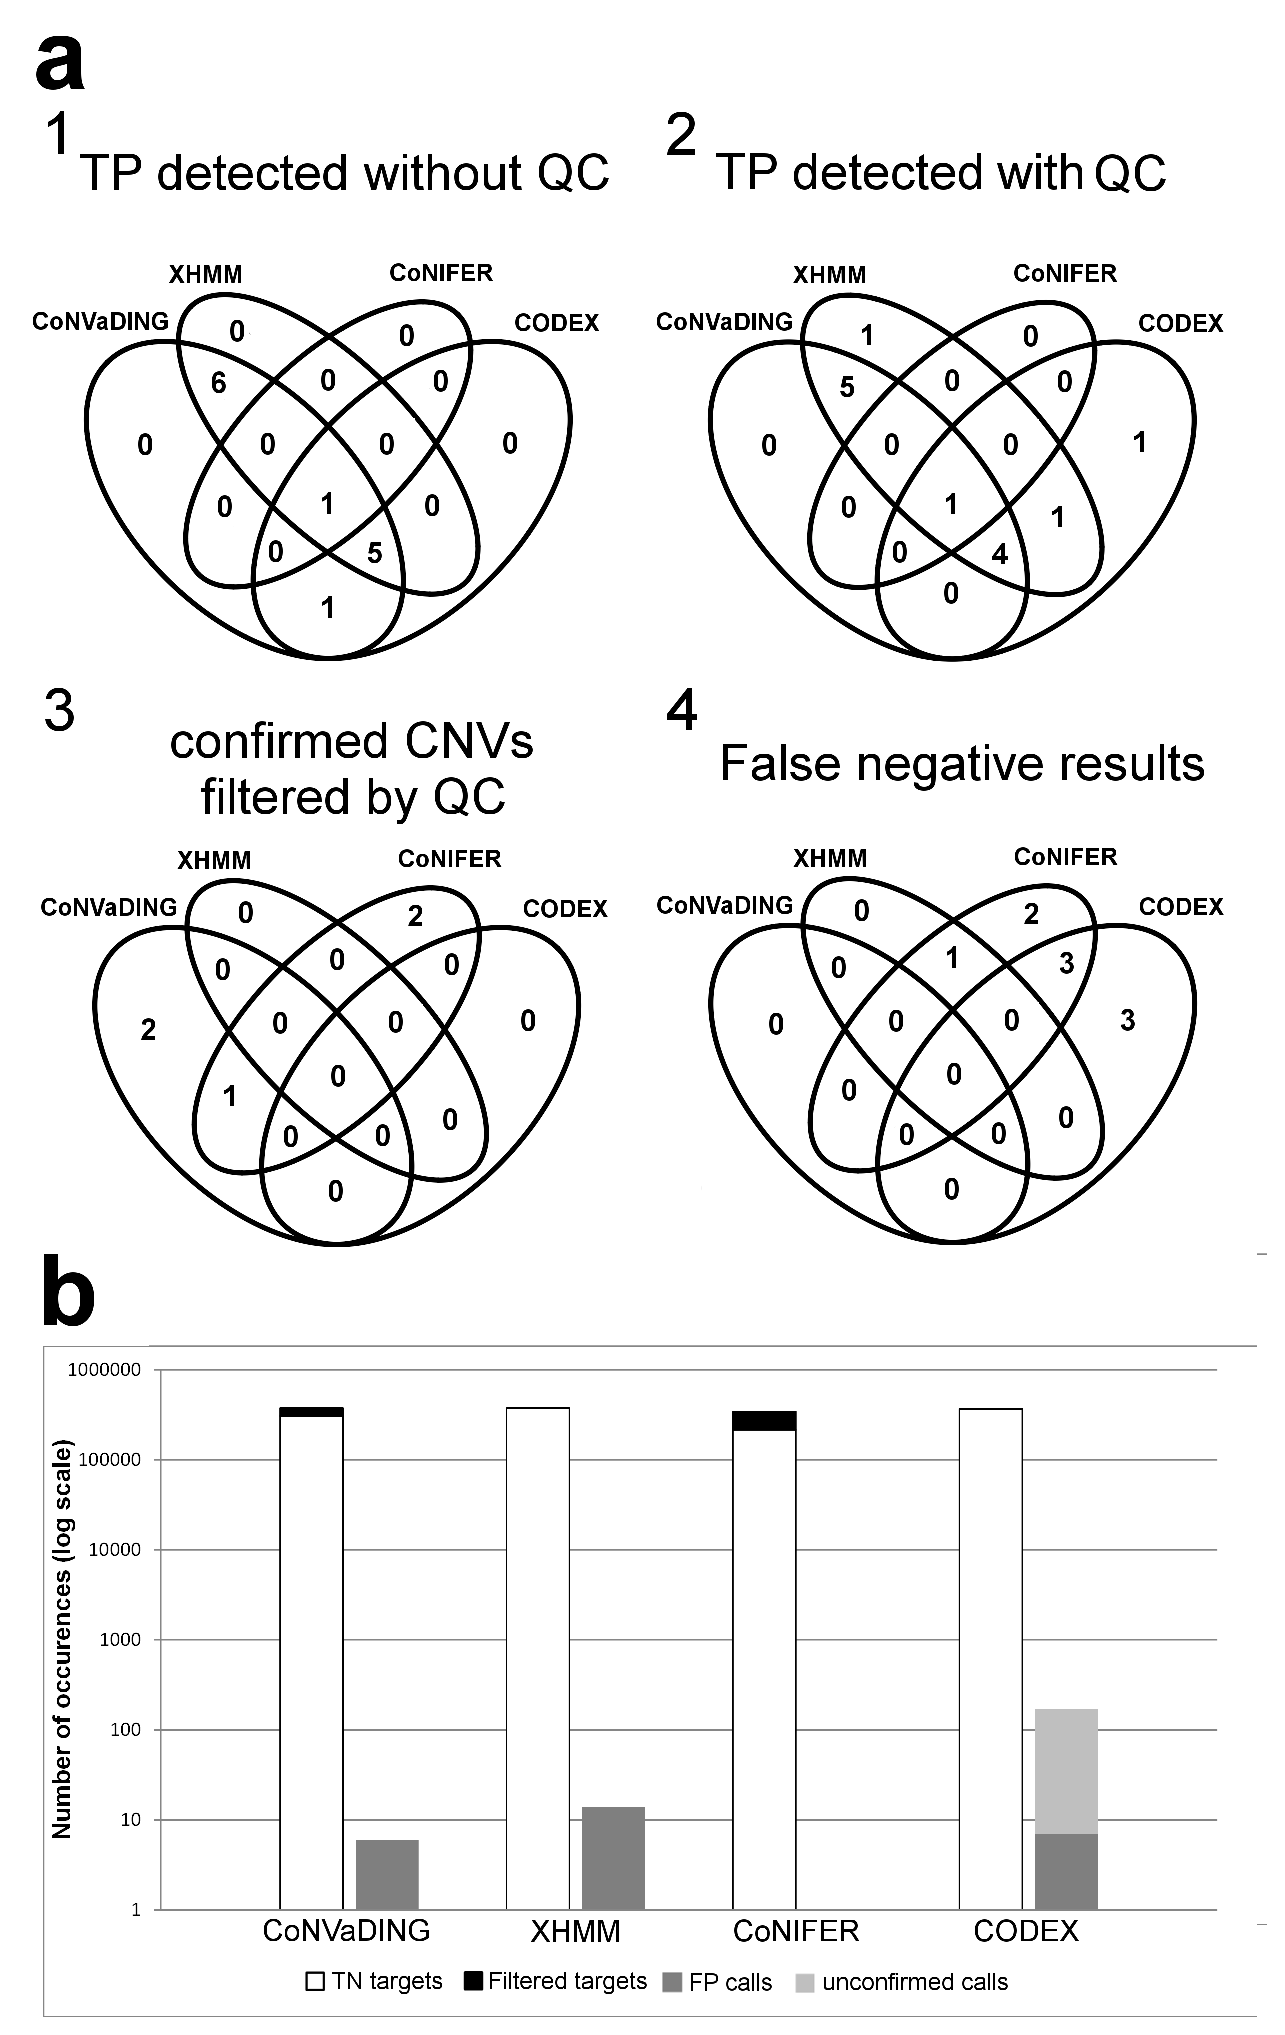
\includegraphics[width=0.9\linewidth]{img/CoNVaDING_Fig3}
	\caption[CNV detections CoNVaDING, XHMM, CoNIFER, and CODEX]{Caption next page.}
	\label{fig:CoNVaDING_Fig3}
\end{figure}
\addtocounter{figure}{-1}
\begin{figure}
	\caption[]{(Previous page.)CNV detections made by CoNVaDING, XHMM, CoNIFER, and CODEX. A: Venn diagrams showing true- positive (TP) and false-negative (FN) calls (1) TP detected without quality control (QC), (2) TP detected with QC, (3) confirmed CNVs filtered by QC, and (4) FN results. B: Bar plot using a log 10 scale showing the true-negative (TN), filtered targets (FT), false-positive (FP) results, and unconfirmed calls.}
\end{figure}

\subsection{Comparison to CoNIFER, XHMM and CODEX}
In the CoNIFER analysis, 42\% of samples failed to pass Sample QC: 31 and 102 for the FC and CM panels, respectively. 
In the remaining samples only one TP CNV (del 5 exons BRCA1) was identified and no additional CNVs were detected. 

In the XHMM analysis, all samples passed Sample QC and only three targets in the FC panel and five in the CM panel failed Target QC. 
Twelve TP and thirteen FP CNVs were called. 
Only one of the FP results, a one exon PLN duplication, was also detected by CoNVaDING. 
XHMM produced one FN result, since it did not detect the 1 exon MSH2 deletion, even though that sample and target had passed QC. 
In the CODEX analysis, all samples passed Sample QC and fourteen targets in the FC panel and thirty in the CM panel failed Target QC. 
In total, seven TP CNVs were called among 165 other calls, 49 in the FC, and 116 in the CM panel, respectively (Supplemental Table S4). 
Of those other calls, 112 calls were found in samples that failed CoNVaDING sample QC, 36 and 76 for the FC and CM panels, respectively. 
Due to the high number of novel calls, we did not confirm CNVs that were called only by CODEX. 
However, six calls were confirmed FP, because these were either called by XHMM or were present on the CoNVaDING shortlist. 
CoNIFER, XHMM, and CODEX analysis resulted in sensitivities of 16.7\%, 92.3\%, and 53.8\% and specificities of 100\%, 99.997\%, and 99.955\%–99.998\%, respectively, for targets passing all QC. 
Ten of the 13 FP findings by XHMM were located in samples or targets that failed CoNVaDING Sample QC or Target QC. 
Supplemental Table S3 shows all CNVs detected by one ormore of the tools. 
A comparison of FP and TN results is shown in Figure  \ref{fig:CoNVaDING_Fig1}B.



\subsection{Performance of CoNVaDING on Low-Coverage Data}
Using default settings, 101 FC and eight CM samples passed
sample QC at an average coverage of 100x and no sample passed sample QC at a coverage of 50x. 
To enable analysis, sample QC thresholds were increased to 0.11 and 0.13 for the 100x and 50x coverage samples, respectively. Using these settings, 117 FC and 179 CM samples passed sample QC at a coverage of 100x. 
These numberswere 112 and 31 for the FC and CM panels, respectively, at 50x coverage. 
At a coverage of 100x, only 60,663 (50\%) and 38,749 (15\%) of the targets analyzed passed all QC for the FC and CM panel, respectively. 
At a coverage of 50x, these numbers were 2,825 (2.3\%) and 1,014 (0.4\%). 
At 100x coverage, eight of the 13 CNVs that were confirmed by MLPA were detected and one remained at a coverage of 50x (Supplemental Table S5).
However, given a target passing both Target QC and Sample QC, the sensitivity stayed at 100\%. Specificity was 99.993\% (seven FP results) and 100\% at a coverage of 100x and 50x, respectively.


\section{Discussion}\label{discussion}
We have developed CoNVaDING, as a tool for detecting single exon CNVs in targeted NGS data. 
CNV detection in targeted NGS data is a challenge, because not every targeted region can be analyzed reliably. 
Therefore, for each target, CoNVaDING determines whether a high sensitivity and specificity can be obtained. 
This is especially important in a clinical diagnostic setting, where it is necessary to know exactly those targets for which a CNV could remain undetected.Adding information about failed targets indicates which targets should be tested using another method and for which targets a deletion or duplication can be detected or ruled out with high confidence. In our validation, we used high-coverage NGS data from targeted gene panels. 
By analyzing all potential CNVs using MLPA, we could validate calls as small as a single exon and accurately determine sensitivity and specificity. After MLPA, we determined a 100\% sensitivity and a 99.998\% specificity for CoNVaDING analysis in targets passing QC. 
Previous validations of XHMM and CoNIFER were based on concordance between SNP array calls and whole-exome sequencing data. 
The validation studies using this approach determined a sensitivity of 67\% for XHMM \cite{Fromer_2012} and 76\%–84\% for CoNIFER \cite{Krumm_2012}. 
In contrast, we found a higher sensitivity for XHMM calls (92.3\%) and much lower sensitivity (16.7\%) for CoNIFER. 
It may be that CoNIFER CNV calling was hampered by the small CNV size in our positive control samples. 
In the previous CODEX validation study, sensitivity was determined using a simulation data set and approached 100\% sensitivity for rare CNVs having a minimum length of five exons \cite{Jiang_2015}. 
In our study, we called three out of four CNVs having five exons or more (75\%) and four out of nine (44.4\%) CNVs smaller than five exons.

Our data show that CoNVaDING outperforms CoNIFER, XHMM, and CODEX because of its QC metrics, making high-coverage NGS gene panel data suitable as first line CNV detection data, regardless of the CNV size. 
CoNVaDING flagged around 10\% of the targets as low quality, indicating that these targets are not suitable for single exon variation detection due to a high variability of that target in the selected control samples. 
However, multiple exon variations containing low-quality targets can still be detected, as long as part of the CNV region is of sufficient quality. 
The moderate numbers of samples and targets flagged as low quality by CoNVaDING, combined with FP XHMM results in these samples and targets, suggest that CoNVaDING quality metrics successfully filter out samples and targets with a higher likelihood of FP results. 
The high number of excluded CoNIFER samples and the absence of failed samples and near absence of failed targets in XHMM and CODEX analysis suggest suboptimal QC performance of these tools. 
Our results also suggest that specificity can be even further improved by combining CoNVaDING with the other algorithms, since there is only a small overlap between FP calls and a high concordance in TP calls (Supplemental Table S3). 
CoNVaDING is primarily designed for detection of rare germline CNVs by targeted sequencing and for use in both research and clinical settings. 
The presence of (common) CNVs in the set of possible control samples may lead CoNVaDING to consider the targets within the CNV region as low quality. 
We determined the effect of a lower coverage on the performance of CoNVaDING. 
Since variability between samples increases at a lower coverage,more targetswere labeled as low quality. 
The number of targets passing QC was considerably higher in the FC than in the CM panel, suggesting that the minimum coverage needed differs per capturing panel. 
Given the results of the analysis of downsampled targets, we expect CoNVaDING to be able to analyze 15\%–50\% of the targets in a 100x coverage exome at a single-exon resolution. 
At a lower resolution, we expect more targets to pass QC. 
We also tested CoNVaDING on low-coverage whole-genome sequencing data (30x average) using 10 kb bins as targets. 
Although the increased bin size lowered the resolution as comparedwith analysis in high coverage data, a high concordance with SNP array data was found for calls larger than 50 kb. 
The extent to which this can be used as a method to detect smaller CNVs is currently being investigated. 
In conclusion, CoNVaDING improves sensitivity and specificity as well as QC for CNV analysis of NGS data. 
Our tool shows not only which CNVs are detected, but also which specific targets are unreliable for CNV analysis. 
We consider CoNVaDING uniquely fit for detection of single exon CNVs in targeted NGS data, making it an indispensable addition to the CNV detection tool box in both research and clinical diagnostic settings.


\section{Acknowledgments}\label{Acknowledgments} 
We thank Jackie Senior and Kate Mc Intyre for editorial advice.


\subsubsection{Disclosure Statement} 
The authors declare no conflict of interest.

\subsubsection{Supplemental Material}
Supplemental methods and tables: \\ https://onlinelibrary.wiley.com/doi/abs/10.1002/humu.22969 \\
\\
CoNVaDING source code and documentation: \\ https://github.com/molgenis/CoNVaDING  \\
\\
CoNVaDING video tutorial: \\ https://www.youtube.com/watch?v=-geFWkvKZzE\&feature=youtu.be